%% Define the document style. The thesis stylesheet inherits from 'report'. 
%% I had once made a version inheriting from book. However the two versions are almost 
%% compatible. The main difference is that the other version supported 'parts'.
%% (extended from book) and this does not.
%% IST requires the thesis to be written in Arial or similar. Two arguments allow you 
%% to define the thesis font: 'Helvetica' and 'AvantGarde', which transforms normal font
%% into Helvetica or AvantGarde, respectively... dahhhh!
\documentclass[defaultstyle,10pt,master,Helvetica]{thesis}
%\documentclass[defaultstyle,12pt,phd]{thesis}

%% STYLESHEET SPECIFIC EXTRA COMMANDS (defined in thesis.cls):
%% ------------------------------------------------------------
%% \fancychapter{chaptername) -> Prints a fancier chapter
%% \hline{width} -> use for a replacement of the \hline command
%% \Mark1, \Mark2, \Mark3, ...

%% Defines an additional alphabet... not required in most cases
%% ------------------------------------------------------------
% \DeclareMathAlphabet{\mathpzc}{OT1}{pzc}{m}{it}

%% PACKAGE babel:
%% ---------------
%% The 'babel' package may correct some hyphenisation issues of latex. 
%% However in most situations it is not required.
% \usepackage[english]{babel}

%% PORTUGUESE WRITTEN DOCUMENTS
%% ---------------
%% If you are writting the document in portuguese you will have to use the following 
%% packages and commands:
% \usepackage[portuges]{babel} 
% \usepackage[fixlanguage]{babelbib}
% \selectbiblanguage{portuges}
% \def\chapterautorefname{Capítulo}
% \def\sectionautorefname{Sec\c{c}\~ao}
% \def\subsectionautorefname{Subsec\c{c}\~ao}
% \def\figureautorefname{Figura}
% \def\tableautorefname{Tabela}

%% SPECIAL LATIN CHARACTERS
%% ---------------
%% During the writting of the document you are likely to have to write some latin 
%% specific characters which are not typically available in english, e.g., vowels 
%% with accents. By default LaTeX2E is not prepared to handle these special characters. 
%% You can however add a package to handle these cases:
%%
%% if you are under linux, using UTF8 encoded characters, apply the following:
\usepackage[utf8]{inputenc}
%% if you are under windows, you will likely require the following package:
%\usepackage[latin1]{inputenc}

%% PACKAGE fontenc:
%% -----------------
%% chooses T1-fonts and allows correct automatic hyphenation.
%\usepackage[T1]{fontenc}

%% PACKAGE latexsym:
%% -----------------
%% Defines additional latex symbols. May be required for thesis with many math symbols.
%\usepackage{latexsym}

%% PACKAGE amsmath, amsthm, amssymb, amsfonts:
%% -------------------------------------------
%% This package is typically required. Among many other things it adds the possibility
%% to put symbols in bold by using \boldsymbol (not \mathbf); defines additional 
%% fonts and symbols; adds the \eqref command for citing equations. I prefer the style
%% "(x.xx)" for referering to an equation than to use "equation x.xx".
\usepackage{amsmath, amsthm, amssymb, amsfonts}

%% PACKAGE multirow, colortbl, longtable:
%% ---------------------------------------
%% These packages are most usefull for advanced tables. The first allows to join rows 
%% throuhg the command \multirow which works similarly with the command \multicolumn
%% The second package allows to color the table (both foreground and background)
%% The third package is only required when tables extend beyond the length of one page;
%% which typically does not happen and should be avoided
\usepackage{multirow}
\usepackage{colortbl}
% \usepackage{longtable}

%% PACKAGE graphics, epsfig, subfigure, caption:
%% ---------------------------------------------
%% Packages for figures... well you will certainly need these packages, with the exception
%% of the 'caption' package. This only allows to define extra caption options.
%% Notice that subfigure allows to place figures within figures with its own caption. It
%% should be avoided to create an eps file with subfigures. That will mean that you won't be 
%% able to reference those subfigures. Instead create an EPS file (the only graphics format supported
%% by latex) for each of the subfigures and then use the command \subfigure (see below).
\usepackage{graphics}
\usepackage{epsfig}
\usepackage[hang,small,bf]{subfigure}
% \usepackage[hang,small,bf]{caption}

%% PACKAGE algorithmic, algorithm
%% ------------------------------
%% These packages are required if you need to describe an algorithm.
% \usepackage{algorithmic}
% \usepackage[chapter]{algorithm}

%% PACKAGE natbib/cite
%% -------------------
%% The two packages are not compatible, and you should use one of the two. Notice however that the
%% IEEE BiBTeX stylesheet is imcompatible with the natbib package. If using the IEEE format, use the 
%% cite package instead
%%
%% For numeric citations use:
\usepackage[square,numbers,sort&compress]{natbib}
%% For numeric author-year use:
% \usepackage[round,authoryear]{natbib}
%% For the cite package instead use:
%\usepackage{cite}

%% PACKAGE acronyum
%% -----------------
%% This package is most usefull for acronyms. The package garantees that all acronyms definitions are 
%% given at the first usage. IMPORTANT: do not use acronyms in titles/captions; otherwise the definition 
%% will appear on the table of contents.
\usepackage[printonlyused]{acronym}

%% PACKAGE hyperref
%% -----------------
%% Set links for references and citations in document
%% Some MiKTeX distributions have faulty PDF creators in which case this package will not work correctly
%% Long live Linux :D
\usepackage{hyperref}
\hypersetup{ a4paper=true,
             colorlinks=false,
             citecolor=red,
             breaklinks=true,
             bookmarks=true,
             bookmarksnumbered=true,
             bookmarksopen=true,
             pdftitle={DOCUMENT TITLE},                 % EDIT THIS LINE
             pdfauthor={THE AUTHOR},                    % EDIT THIS LINE
             pdfsubject={THE SUBJECT},                  % EDIT THIS LINE
             pdfcreator={THE PDF CREATOR - THE AUTHOR}, % EDIT THIS LINE
             pdfkeywords={}                             % EDIT THIS LINE
}

%% Set paragraph counter to alphanumeric mode
\renewcommand{\theparagraph}{\Alph{paragraph}~--}

%% Page formatting... It was correct for my master thesis... not sure it is still correct
%% edit as necessary
\hoffset 0in
\voffset 0in
\oddsidemargin 0.71cm
\evensidemargin 0.04cm
\marginparsep 0in
\topmargin -0.25cm
\textwidth 15cm
\textheight 23.5cm

\usepackage{fancyhdr}
\pagestyle{fancy}
\renewcommand{\chaptermark}[1]{\markboth{\thechapter.\ #1}{}}
\renewcommand{\sectionmark}[1]{\markright{\thesection\ #1}}
\fancyhf{} \fancyhead[LE]{\bfseries\nouppercase{\leftmark}}
\fancyhead[RO]{\bfseries\nouppercase{\rightmark}}
\fancyfoot[LE,RO]{\bfseries\thepage}
\renewcommand{\headrulewidth}{0.5pt}
\renewcommand{\footrulewidth}{0.5pt}
\addtolength{\headheight}{2pt} % make space for the rule
\fancypagestyle{plain}{%
   \fancyhead{} % get rid of headers
   \renewcommand{\headrulewidth}{0pt} % and the line
   \renewcommand{\footrulewidth}{0pt}
}
\fancypagestyle{blank}{%
   \fancyhf{} % get rid of headers and footers
   \renewcommand{\headrulewidth}{0pt} % and the line
   \renewcommand{\footrulewidth}{0pt}
}
\fancypagestyle{abstract}{%
   \fancyhead{}
   \renewcommand{\headrulewidth}{0pt}
   \renewcommand{\footrulewidth}{0.5pt}
}
\fancypagestyle{document}{%
	\fancyhf{} \fancyhead[LE]{\bfseries\nouppercase{\leftmark}}
	\fancyhead[RO]{\bfseries\nouppercase{\rightmark}}
	\fancyfoot[LE,RO]{\bfseries\thepage}
	\renewcommand{\headrulewidth}{0.5pt}
	\renewcommand{\footrulewidth}{0.5pt}
	\addtolength{\headheight}{2pt} % make space for the rule
}
\setcounter{secnumdepth} {5}
\setcounter{tocdepth} {5}
\renewcommand{\thesubsubsection}{\thesubsection.\Alph{subsubsection}}

\renewcommand{\subfigtopskip}{0.3 cm}
\renewcommand{\subfigbottomskip}{0.2 cm}
\renewcommand{\subfigcapskip}{0.3 cm}
\renewcommand{\subfigcapmargin}{0.2 cm}


\begin{document}

% Add PDF bookmark 
\pdfbookmark[0]{Titlepage}{Title}

%%%%%%%%%%%%%%%%%%%%%%%%%%%%%%%%%%%%%%%%%%%%%%%%%%%%%%%%%%%%%%%%%%%%%%%%%%%%%%%%%%%%%%%%%%%%%%%%
% DEFINE THE TITLEPAGE
% remember that IST requires for the titlepage to be written in portuguese
%%%%%%%%%%%%%%%%%%%%%%%%%%%%%%%%%%%%%%%%%%%%%%%%%%%%%%%%%%%%%%%%%%%%%%%%%%%%%%%%%%%%%%%%%%%%%%%%
% REQUIRED:
% The university logo image: first and second arguments are the (top,left) position of the logo. 
% IST rules force it to be 2cm
\univlogo{3cm}{2cm}{logo_ist_web.eps}
% OPTIONAL:
% The thesis logo image: first and second arguments are the position of the logo. 
\thesislogo{2.5cm}{6cm}{thesis_logo.eps}

% Thesis title
\title{A IST stylesheet example for writing dissertations}

% Author and highest current degree (not the one you are applying to)
\author{Pedro Tom\'as}
\degree{Engenharia Electrot\'ecnica e de Computadores}
% This is not on the new IST MSc stylesheet... however for PhD dissertations it will most likely be required
% \otherdegree{Mestre}

% The supervisor. Use the second command if required.
% Always remember that 'Professor' should only be used for a supervisor with a Cathedra
\supervisor{Doutor full name of advisor}
% \othersupervisor{Doutor full name of co-advisor}

% Date of the dissertation
\date{Julho de 2007}

% Is this the final version? Place false when delivering the first part.
% The juri members will not be printed in that case. Place true after the juri has accepted the thesis
\finalthesis{true}

% The members of the Juri
% Always remember that 'Professor' should only be used for a juri member with a Cathedra
\presidentofjury{Doutor whatever full name 1}
\vogalone{Doutor whatever full name 2}
\vogaltwo{Doutor whatever full name 3}
% \vogalthree{Doutor whatever full name 4}
% \vogalfour{Doutor whatever full name 5}
%%%%%%%%%%%%%%%%%%%%%%%%%%%%%%%%%%%%%%%%%%%%%%%%%%%%%%%%%%%%%%%%%%%%%%%%%%%%%%%%%%%%%%%%%%%%%%%%

% print titlepage
\maketitle
\clearpage

% Since I am using double sided pages, the second page should be white.
% Remember that when delivering the dissertation, IST requires for the cover to appear twice.
\thispagestyle{empty}
\cleardoublepage

\setcounter{page}{1} \pagenumbering{roman}

\baselineskip 18pt % line spacing: -12pt for single spacing
                   %               -18pt for 1 1/2 spacing
                   %               -24pt for double spacing

\pdfbookmark{Acknowledgments}{Acknowledgments}
\begin{acknowledgments}
Thanks to the author of this document... If you are not thanking than... you are not thanking!!!
\end{acknowledgments}

\pdfbookmark{Abstract}{Abstract}
\begin{abstract}
Place your abstract in here
\end{abstract}

\begin{keywords}
Put 6 keywords in here
\end{keywords}
\clearpage
\thispagestyle{empty}
\cleardoublepage

\pdfbookmark{Resumo}{Resumo}
\begin{resumo}
Place your abstract in here... in portuguese now
\end{resumo}

\begin{palavraschave}
Put 6 keywords in here... in portuguese now
\end{palavraschave}

\clearpage
\thispagestyle{empty}
\cleardoublepage

% This is required for the fancy chapters
\dominitoc
\dominilof
\dominilot

%%%%%%%%%%%%%%%%%%%%%%%%%%%%%%%%%%%%%%%%%%%%%%%%%%%%%%%%%%%%%%%%%%%%%%
% List of contents
%\renewcommand{\baselinestretch}{1}
\pdfbookmark[0]{Index}{index}
\pdfbookmark[1]{Contents}{toc}
\tableofcontents
% \contentsline{chapter}{References}{\pageref{bib}}
\cleardoublepage
%\renewcommand{\baselinestretch}{1.5}

%%%%%%%%%%%%%%%%%%%%%%%%%%%%%%%%%%%%%%%%%%%%%%%%%%%%%%%%%%%%%%%%%%%%%%
% List of figures
\pdfbookmark[1]{List of Figures}{lof}
\listoffigures
\cleardoublepage

%%%%%%%%%%%%%%%%%%%%%%%%%%%%%%%%%%%%%%%%%%%%%%%%%%%%%%%%%%%%%%%%%%%%%%
% List of tables
\pdfbookmark[1]{List of Tables}{lot}
\listoftables
\cleardoublepage

% %%%%%%%%%%%%%%%%%%%%%%%%%%%%%%%%%%%%%%%%%%%%%%%%%%%%%%%%%%%%%%%%%%%%%%
% % List of algorithms
% Requires packages algorithmic, algorithm
% \pdfbookmark[1]{List of Algorithms}{loa}
% \listofalgorithms
% \cleardoublepage

% %%%%%%%%%%%%%%%%%%%%%%%%%%%%%%%%%%%%%%%%%%%%%%%%%%%%%%%%%%%%%%%%%%%%%%
% % List of acronyms
% \pdfbookmark[1]{List of Acronyms}{loac}
% \input{acronim.tex}

% Pages number is starting now with arabic style... until now it was on roman mode
\setcounter{page}{1} \pagenumbering{arabic}
\baselineskip 18pt

% %%%%%%%%%%%%%%%%%%%%%%%%%%%%%%%%%%%%%%%%%%%%%%%%%%%%%%%%%%%%%%%%%%%%%%
% The Introduction:
% %%%%%%%%%%%%%%%%%%%%%%%%%%%%%%%%%%%%%%%%%%%%%%%%%%%%%%%%%%%%%%%%%%%%%%
% Notice that I am using my own chapter style, instead of the default one
\fancychapter{Introduction}
Write your introduction in here. You should start by introducing your thesis in a way that the reader understands where your thesis stand in todays technology and overall knowledge. Consider answering questions such as:
\begin{enumerate}
 \item what is the background of your work?
 \item how do your work fit in todays knowledge? Have you done something that does not exist in the market? What are the differences? What is missing in nowadays products and solutions?
 \item is your thesis made as part of a larger project? If so, describe it.
 \item is your thesis usefull for some work environment? If so, describe it.
\end{enumerate}

\section{Motivation}

Given the general description provided previously, what is the motivation of your work. Explain why the product or solution developed in the course of your thesis is important.

\section{Objectives}

This section should describe the objectives of your work.

\section{Main contributions}
Do not forget this one. Notice that the objectives is what you have proposed to do. Main contributions are the innovations of your work, or, in other cases, what your work is really good at. If you submitted/published an article in a peer-reviewed conference or journal, do not forget to state here.

\section{Dissertation outline}

Explain how did you organized your thesis.

% If you prefer to have multiple files, each storing, for example, a different chapter (or a section within a chapter)
% you can use one of the following commands:
%
% \input{my_tex_file.tex}
% \include{my_tex_file.tex}
% 
% the difference between the two commands is that \include will always start a new page, whereas \input does not

\cleardoublepage

% %%%%%%%%%%%%%%%%%%%%%%%%%%%%%%%%%%%%%%%%%%%%%%%%%%%%%%%%%%%%%%%%%%%%%%
% State of the art
% %%%%%%%%%%%%%%%%%%%%%%%%%%%%%%%%%%%%%%%%%%%%%%%%%%%%%%%%%%%%%%%%%%%%%%
\fancychapter{State of the art}
The second chapter can be the state of the art for the work you are preenting. Sometimes it appears under the previous chapter -- Introduction. Though I typically prefer to put it in a separate chapter.

In most cases this chapter addresses some important technology or knowledge. Name this chapter according to the topic.

The introduction should be written assuming that the reader has little or no knowledge of your specific problem. Try to write this chapter in a clear manner that makes it easier for the reader to understand the remaining of your thesis. Append information to this chapter as needed when writting other chapters.

Do not forget to add references to your document. In general, if you are stating something which is not obvious nor it is of common knowledge amongst the scientific or engineering community, you should place a reference. To ease the process of referencing I include a couple of references to my own papers herein. Here are some examples: \cite{tomas2010bda}, \citep{tomas2010aqa}, \citet{ramalho2010eic}, \mbox{\cite[(2.2)]{tomas2009nct}}.

To help you make references, you can try the commands or consult the manual. The following link can also be a good help:
\mbox{\underline{http://merkel.zoneo.net/Latex/natbib.php}}.

As a side note, remember that you should not include links in your dissertation as I just made. Instead you should put a reference as follows: \cite{mylink}. Remember that in this case, the reference date is the date you have last consulted the page.

\section{Summary}

It is typical a good ideia to have an ending section summarizing the chapter.

% Ensure that the next chapter starts in a odd page
\cleardoublepage

% %%%%%%%%%%%%%%%%%%%%%%%%%%%%%%%%%%%%%%%%%%%%%%%%%%%%%%%%%%%%%%%%%%%%%%
% Your work: Chapter 1
% %%%%%%%%%%%%%%%%%%%%%%%%%%%%%%%%%%%%%%%%%%%%%%%%%%%%%%%%%%%%%%%%%%%%%%
\fancychapter{The work}

{\color{red}\bfseries IMPORTANT NOTICE: This chapter should not be called ``The Work'' in the final version of your dissertation. This comment was inserted after some of my faculty collegues noticed that some naive souls call the chapter ``The Work''. This is by no means appropriate. This and all chapter names should be named accordingly to your thesis.}

The third chapter is typically the work you have performed in your thesis. Obviously you should focus on your contributions, but do not forget to write it so that others can understand. Never assume the reader knows the subject (unless it is really obvious). Your work is typically done in a very specific area which others may not know as much. So try to make it as clear as possible; and a self-explaining figure is always a big help.

\begin{figure}[t]
\centering
\subfigure[caption for subfigure a]{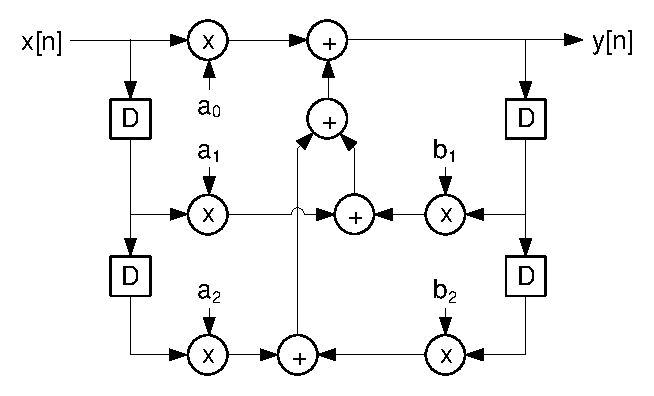
\includegraphics[scale=0.65]{img1.eps}\label{chp3:img1}}
\hspace*{0.5cm}
\subfigure[caption for subfigure b]{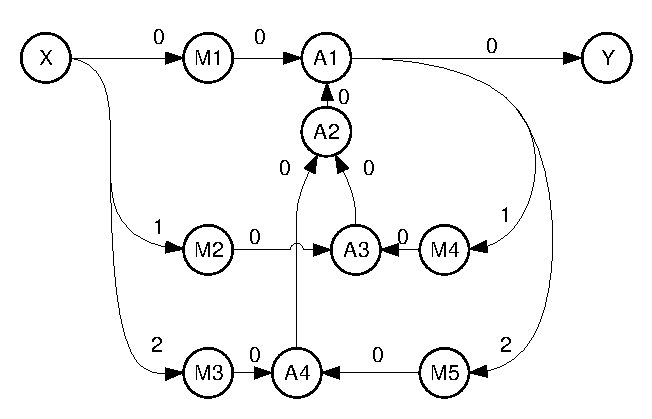
\includegraphics[scale=0.65]{img2.eps}\label{chp3:img2}}\\
\caption{A figure example.}
\label{fig:rmain figure}
\end{figure}

See the source code to see how to reference each of the subfigures \ref{chp3:img1} or \ref{chp3:img2}, or the main figure \ref{fig:rmain figure}.

There are several ways to define formulas (see the \textit{Short Math Guide for LaTeX} included in the package). The typical method is to use (see source code): 
\begin{equation}
a= b + c
\end{equation}
or
\begin{align}
c &= d \cdot e \nonumber\\
d &= \mathbf{X}^{\mathsf{T}} \mathbf{Y}+ \gamma e^{2\pi}
\label{chp3:eq1} 
\end{align}
or
\begin{subequations}
\begin{align}
c &= d \cdot e \label{chp3:eq2:a} \\
d &= \mathbf{X}^{\mathsf{T}} \mathbf{Y} + \gamma e^{2\pi}
\label{chp3:eq2:b} 
\end{align}
\label{chp3:eq2} 
\end{subequations}
where $\mathbf{X}$ and $\mathbf{Y}$ are column vectors (you should always present the meaning of each parameter). The \textbf{AMS} packages allow to use the command \verb"\eqref" to cite equations such as \eqref{chp3:eq1},  \eqref{chp3:eq2:a},\eqref{chp3:eq2:b} or \eqref{chp3:eq2} (see source code).

\section{Summary}

It is typical a good ideia to have an ending section summarizing the chapter.

% Ensure that the next chapter starts in a odd page
\cleardoublepage

% %%%%%%%%%%%%%%%%%%%%%%%%%%%%%%%%%%%%%%%%%%%%%%%%%%%%%%%%%%%%%%%%%%%%%%
% Your work: Chapter 2
% %%%%%%%%%%%%%%%%%%%%%%%%%%%%%%%%%%%%%%%%%%%%%%%%%%%%%%%%%%%%%%%%%%%%%%
\fancychapter{Implementation}
While the first chapter focus on your ideas the second can focus on the implementation. Though that may change from thesis to thesis.

\begin{figure}
\begin{boxedverbatim}
DefineGlobals
   clock   alias   clk
   reset   alias   rst
   max_latency     17
   feedback        0
   DefineInputs
      X   std_logic_vector(11 downto 0)
   EndInputs
   DefineOutputs
      Y   std_logic_vector(11 downto 0)
   EndOutputs
EndGlobals
\end{boxedverbatim}
\caption{An example code section.}
\label{chp4:img}
\end{figure}

Figure~\ref{chp4:img} shows an example of a \verb"\boxedverbatim" section. It allows to put blocks of code within a frame. I think makes a prettier printing.

\section{Summary}

It is typical a good ideia to have an ending section summarizing the chapter.

% Ensure that the next chapter starts in a odd page
\cleardoublepage

% %%%%%%%%%%%%%%%%%%%%%%%%%%%%%%%%%%%%%%%%%%%%%%%%%%%%%%%%%%%%%%%%%%%%%%
% Experimental results
% %%%%%%%%%%%%%%%%%%%%%%%%%%%%%%%%%%%%%%%%%%%%%%%%%%%%%%%%%%%%%%%%%%%%%%
\fancychapter{Results}
\section{Testing framework}
For helping the reader first explain how did you achieve your experimental results. This may include (but is not limited to): the algorithm parameters; the computer or harware platform performing the operations; the comparative algorithms, frameworks or platforms parameters.

% use include if you want a page break at the end of the included tex.
\newcommand{\greyrow}{\rowcolor[rgb]{0.9,0.9,0.9}}
\newcommand{\whiterow}{\rowcolor[rgb]{1,1,1}}
\newcommand{\greycell}[1]{\multicolumn{1}{{>{\columncolor[rgb]{0.9,0.9,0.9}}c}}{#1}}
\newcommand{\lightgreycell}[1]{\multicolumn{1}{{>{\columncolor[rgb]{0.9,0.9,0.9}}c}}{#1}}
\newcommand{\mediumgreycell}[1]{\multicolumn{1}{{>{\columncolor[rgb]{0.8,0.8,0.8}}c}}{#1}}
\newcommand{\darkgreycell}[1]{\multicolumn{1}{{>{\columncolor[rgb]{0.7,0.7,0.7}}c}}{#1}}
\newcommand{\whitecell}[1]{\multicolumn{1}{{>{\columncolor[rgb]{1,1,1}}c}}{#1}}

\newcommand{\cellformatG}[1]{\multicolumn{1}{{>{\columncolor[rgb]{.9,.9,.9}}c}}{#1}}
\newcommand{\cellformatW}[1]{\multicolumn{1}{{>{\columncolor[rgb]{1,1,1}}c}}{#1}}
\newcommand{\cellformatlG}[1]{\multicolumn{1}{{|>{\columncolor[rgb]{.9,.9,.9}}c}}{#1}}
\newcommand{\cellformatlW}[1]{\multicolumn{1}{{|>{\columncolor[rgb]{1,1,1}}c}}{#1}}
\newcommand{\cellformatrG}[1]{\multicolumn{1}{{>{\columncolor[rgb]{.9,.9,.9}}c|}}{#1}}
\newcommand{\cellformatrW}[1]{\multicolumn{1}{{>{\columncolor[rgb]{1,1,1}}c|}}{#1}}
\newcommand{\cellformatlrG}[1]{\multicolumn{1}{{|>{\columncolor[rgb]{.9,.9,.9}}c|}}{#1}}
\newcommand{\cellformatlrW}[1]{\multicolumn{1}{{|>{\columncolor[rgb]{1,1,1}}c|}}{#1}}

\begin{table}[t]
\centering
\caption{Example table}
\label{table:table1}
\begin{tabular}{c c c c c c}
\hlinew{0.08cm}
\cellformatrG{}&\cellformatlG{}&\cellformatrG{}&\cellformatlG{}&\cellformatrG{}&\cellformatlG{}\\
\cellformatrG{}&
\cellformatlG{\multirow{-2}{*}{\centering\bf \#Layers}} & 
\cellformatrG{\multirow{-2}{*}{\centering\bf \#Nets}} & 
\cellformatlG{\multirow{-2}{*}{\centering \#Nodes\Mark1}} & 
\cellformatrG{\multirow{-2}{1.8cm}{\centering Critical path}}&
\cellformatlG{\multirow{-2}{2cm}{\centering\bf Latency ($T_{iter}$)}}\\
\cellformatrG{\multirow{-3}{2.2cm}{\centering Benchmark: ANN}} &
\cellformatlG{\footnotesize $(1)$} & 
\cellformatrG{\footnotesize$(2)$} & 
\cellformatlG{\footnotesize$(3)=8\cdot(1)\cdot(2)$} & 
\cellformatrG{\footnotesize$(4)=4\cdot(1)$} & 
\cellformatlG{\footnotesize$(5)$}\\
\hlinew{0.04cm}
\cellformatrW{A1} & \cellformatlW{\bf 3--1501} & \cellformatrW{       1   } & \cellformatlW{\bf 24--12008}  & \cellformatrW{\bf 12--6004} & \cellformatlW{    4}\\
\cellformatrW{A2} & \cellformatlW{    501    } & \cellformatrW{       1   } & \cellformatlW{     4008    }  & \cellformatrW{  2004      } & \cellformatlW{\bf 2--2000 }\\
\cellformatrW{A3} & \cellformatlW{     10    } & \cellformatrW{\bf 2--1024} & \cellformatlW{\bf 160--81920} & \cellformatrW{    40      } & \cellformatlW{   60\Mark2 }\\
\cellformatrW{A4} & \cellformatlW{     10    } & \cellformatrW{      50   } & \cellformatlW{     4000    }  & \cellformatrW{    40      } & \cellformatlW{\bf 80--1200}\\
\hlinew{0.08cm}
\multicolumn{6}{c}{\vspace*{-0.3cm}}\\
%%%%%%%%%%%%% SECOND PART OF THE TABLE %%%%%%%%%%%%%%%%%%%%%%%%
\hlinew{0.08cm}
\cellformatrG{}&\cellformatlG{}&\cellformatrG{}&\cellformatlG{}&\cellformatrG{}&\cellformatlG{}\\
\cellformatrG{}&
\cellformatlG{\multirow{-2}{1.6cm}{\centering\bf FFT size\Mark3}} & 
\cellformatrG{\multirow{-2}{*}{\centering\it\#Inputs}} & 
\cellformatlG{\multirow{-2}{*}{\centering\it \#Nodes\Mark1}} & 
\cellformatrG{\multirow{-2}{1.8cm}{\centering\it Critical path}}&
\cellformatlG{\multirow{-2}{2cm}{\centering\bf Latency ($T_{iter}$)}}\\
\cellformatrG{\multirow{-3}{2.2cm}{\centering Benchmark: FFT}}& 
\cellformatlG{\footnotesize$(1)$} & 
\cellformatrG{\footnotesize$(2)=2^{(1)}$} & 
\cellformatlG{\footnotesize$(3)=10\cdot(1)\cdot (2)$} & 
\cellformatrG{\footnotesize$(4)=4\cdot (1)$} & 
\cellformatlG{\footnotesize$(5)$}\\
\hlinew{0.04cm}
\cellformatrW{F1} & \cellformatlW{\bf 1--10} & \cellformatrW{2--1024} & \cellformatlW{\bf 20--102400} &  \cellformatrW{4--40} & \cellformatlW{6--60\Mark2}\\
\cellformatrW{F2} & \cellformatlW{\bf 5} & \cellformatrW{32} & \cellformatlW{1600} & \cellformatrW{20} & \cellformatlW{\bf 40 -- 1500}\\
\hlinew{0.08cm}
\multicolumn{6}{c}{\vspace*{-0.3cm}}\\
% THIRD AND LAST TABLE!!!
\hlinew{0.08cm}
\cellformatrG{}&\cellformatlG{}&\cellformatrG{}&\cellformatlG{}&\cellformatrG{}&\cellformatlG{}\\
\cellformatrG{}&
\cellformatlG{\multirow{-2}{*}{\centering\bf\#Types}} & 
\cellformatrG{\multirow{-2}{*}{\centering\bf \#Nodes}} & 
\cellformatlG{\multirow{-2}{*}{\centering\it \#Networks}} & 
\cellformatrG{\multirow{-2}{1.8cm}{\centering\it Critical path}}&
\cellformatlG{\multirow{-2}{2cm}{\centering\bf Latency ($T_{iter}$)}}\\
\cellformatrG{\multirow{-3}{2.2cm}{\centering Benchmark: Random networks}}& 
\cellformatlG{\footnotesize$(1)$} & 
\cellformatrG{\footnotesize$(2)$} & 
\cellformatlG{\footnotesize$(3)$} &
\cellformatrG{\footnotesize$(4)$} & 
\cellformatlG{\footnotesize$(5)$}\\
\hlinew{0.04cm}
\cellformatrW{R1} & \cellformatlW{3} & \cellformatrW{10--2000} & \cellformatlW{500} &  \cellformatrW{\it variable} & \cellformatlW{\footnotesize$(4)$}\\
\cellformatrW{R2} & \cellformatlW{3} & \cellformatrW{  50    } & \cellformatlW{500} &  \cellformatrW{\it variable} & \cellformatlW{\footnotesize$(4)\times [1;\cdots;20]$}\\
\hlinew{0.08cm}
\multicolumn{6}{c}{\vspace*{-0.3cm}}\\
\multicolumn{6}{l}{\it\Mark1 Excluding constant nodes.}\\
\multicolumn{6}{l}{\it\Mark2 Value kept proportional to the critical path: $(5)=(4)*1.5$.}\\
\multicolumn{6}{l}{\it\Mark3 A size of $x$ corresponds to a $2^x$ point FFT.}\\
\multicolumn{6}{l}{\it Values in bold indicate the parameter being varied.}
\end{tabular}
\end{table}


For a table example see the file \verb"table_example.tex". It will print table~\ref{table:table1}. Always remember that, unlike with figures, the caption should appear above the table (not below). Also, always remember that the command \verb"\label" should always appear after the command \verb"\caption". If you place it before the caption, the reference will not appear correctly.

\section{The results}
There is usual a future work section as well
As usual you should finish your thesis with the experimental results.

\section{Summary}

It is typical a good ideia to have an ending section summarizing the chapter.

% Ensure that the next chapter starts in a odd page
\cleardoublepage

% %%%%%%%%%%%%%%%%%%%%%%%%%%%%%%%%%%%%%%%%%%%%%%%%%%%%%%%%%%%%%%%%%%%%%%
% Conclusions
% %%%%%%%%%%%%%%%%%%%%%%%%%%%%%%%%%%%%%%%%%%%%%%%%%%%%%%%%%%%%%%%%%%%%%%
\fancychapter{Conclusions}
Draw your conclusions here and sell your work. It is your job to trasmit to the juri how hard it was to develop the presented work. I Good strategy 


\section{Future work}
There is usual a future work section as well

% Ensure that the next chapter starts in a odd page
\cleardoublepage

% Add the Bibliography to the PDF table of contents (not the document table of contents)
\pdfbookmark[0]{Bibliography}{bib}
% The bibliography style sheet
% \bibliographystyle{IEEEtran}
\bibliographystyle{apalike}
% \bibliographystyle{unsorted}
% The BiBTeX file
\bibliography{biblio}
\cleardoublepage

\appendix
% %%%%%%%%%%%%%%%%%%%%%%%%%%%%%%%%%%%%%%%%%%%%%%%%%%%%%%%%%%%%%%%%%%%%%%
% First appendix
% %%%%%%%%%%%%%%%%%%%%%%%%%%%%%%%%%%%%%%%%%%%%%%%%%%%%%%%%%%%%%%%%%%%%%%
\fancychapter{Appendix A}
\cleardoublepage

% %%%%%%%%%%%%%%%%%%%%%%%%%%%%%%%%%%%%%%%%%%%%%%%%%%%%%%%%%%%%%%%%%%%%%%
% Second appendix
% %%%%%%%%%%%%%%%%%%%%%%%%%%%%%%%%%%%%%%%%%%%%%%%%%%%%%%%%%%%%%%%%%%%%%%
\fancychapter{Appendix A}
\cleardoublepage

\end{document}
